\documentclass[]{article}

\usepackage{epigraph}
\usepackage{setspace}
\usepackage{changepage}
\usepackage{amssymb}
\usepackage{amsmath}
\usepackage{graphicx}
%\usepackage{hyperref}
\usepackage[backend=bibtex]{biblatex}
\addbibresource{refs.bib}
%opening
\title{Using A Function Derived From Darts to Visualize Global Optimization Algorithms}
\author{Max Caragozian}


\newcommand{\mustar}{\ensuremath{\mu^* }}
\newcommand{\fmusig}{\ensuremath{F(\mu \vert \sigma)}}

\begin{document}

\maketitle


\epigraph{The tap-room fire is alight again and a new stock of darts laid in; serviceable and well-feathered, that fly true and will see us into another spring.}{``A Chiltern Autumn'' \cite{1929spectator}}

\section{Introcudction}
I bought a dartboard for my college house this past January, and darts quickly became a common pastime during what ended up being a long, snowy winter. I started reading into the mathematics of darts and came across the paper ``A Statistician Plays Darts'' by \citeauthor{stat}\cite{stat}. The paper quantifies how a dart thrower's skill affects where he/she should aim. 

In the simplest model, the authors assume that a person throws with a symmetrical bivariate normal distribution. They estimate the function $\mu^*(\sigma)$ that takes in a standard deviation $\sigma$ and outputs a point $\mu$ that maximizes the expected score of a dart thrown with distribution $\mathcal{N}(\mu, \sigma^2)$.

The authors found that a person with a very small standard deviation should aim for the triple 20 (T20), which shouldn't be surprising as it has the highest point value on the board. The optimal aiming location stays in the T20 until approximately $\sigma=16.9$mm, where the optimal location jumps to the T19, before eventually moving towards the center of the board.

This project compares four different ways to replicate that result.

\begin{figure}
	\centering
	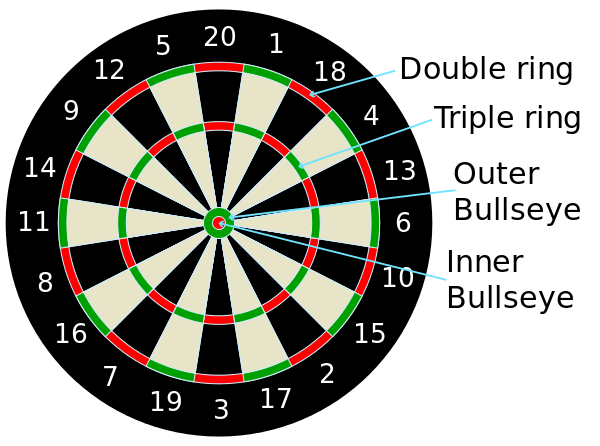
\includegraphics[width=0.8\textwidth]{../images/dartboard_diagram.png}
	\caption{Standard dartboard with point values \cite{diag}}
	\label{fig:diag}
\end{figure}

\section{Integration Brute Force}
Before trying to find $\mu^*(\sigma)$, I wrote code that would find the expected score for someone throwing a dart with a given random distribution. We define a \textit{sector} as a continguous area of the dartboard with a single point value. Examples are the triple 20, the double bullseye, or the portion of single 19 that lies between the outer bullseye ring and the inner triple ring. Let $S$ be the set of all sectors and $X$ be a distribution with PDF $f_x$. To find the expected score of a distribution we compute:



\begin{equation}
	E[score(X)] = \sum_{s \in S} \iint_{s} score_s \cdot  f_x(x, y)  dxdy.
	\label{eq:int}
\end{equation}

I used SciPy's \textit{nquad} function to perform the integration. Originally, I used the \textit{dblquad} method, which is specific to double integral, but I ran into a rounding issues when $f_x$ was very small. The \textit{nquad} function allows finer control and fixed the issue. 

Turning now to the specific case of symmetrical bivariate normal distributions,  let us define the function that takes in a point $\mu$ and returns the expected score of a dart thrown with distribution $\mathcal{N}(\mu, \sigma^2)$ as
\begin{equation}
	F(\mu \vert \sigma).
	\label{eq:fmusig}
\end{equation}
With the code implementation of Equation \ref{eq:int}, I could calculate \fmusig for a grid of possible $\mu$ values across the dartboard. I could then both plot the grid as a heatmap and return the maximum calculated value as a numerical approximation for $\mu^*(\sigma)$.

\begin{figure}[h]
	\centering
	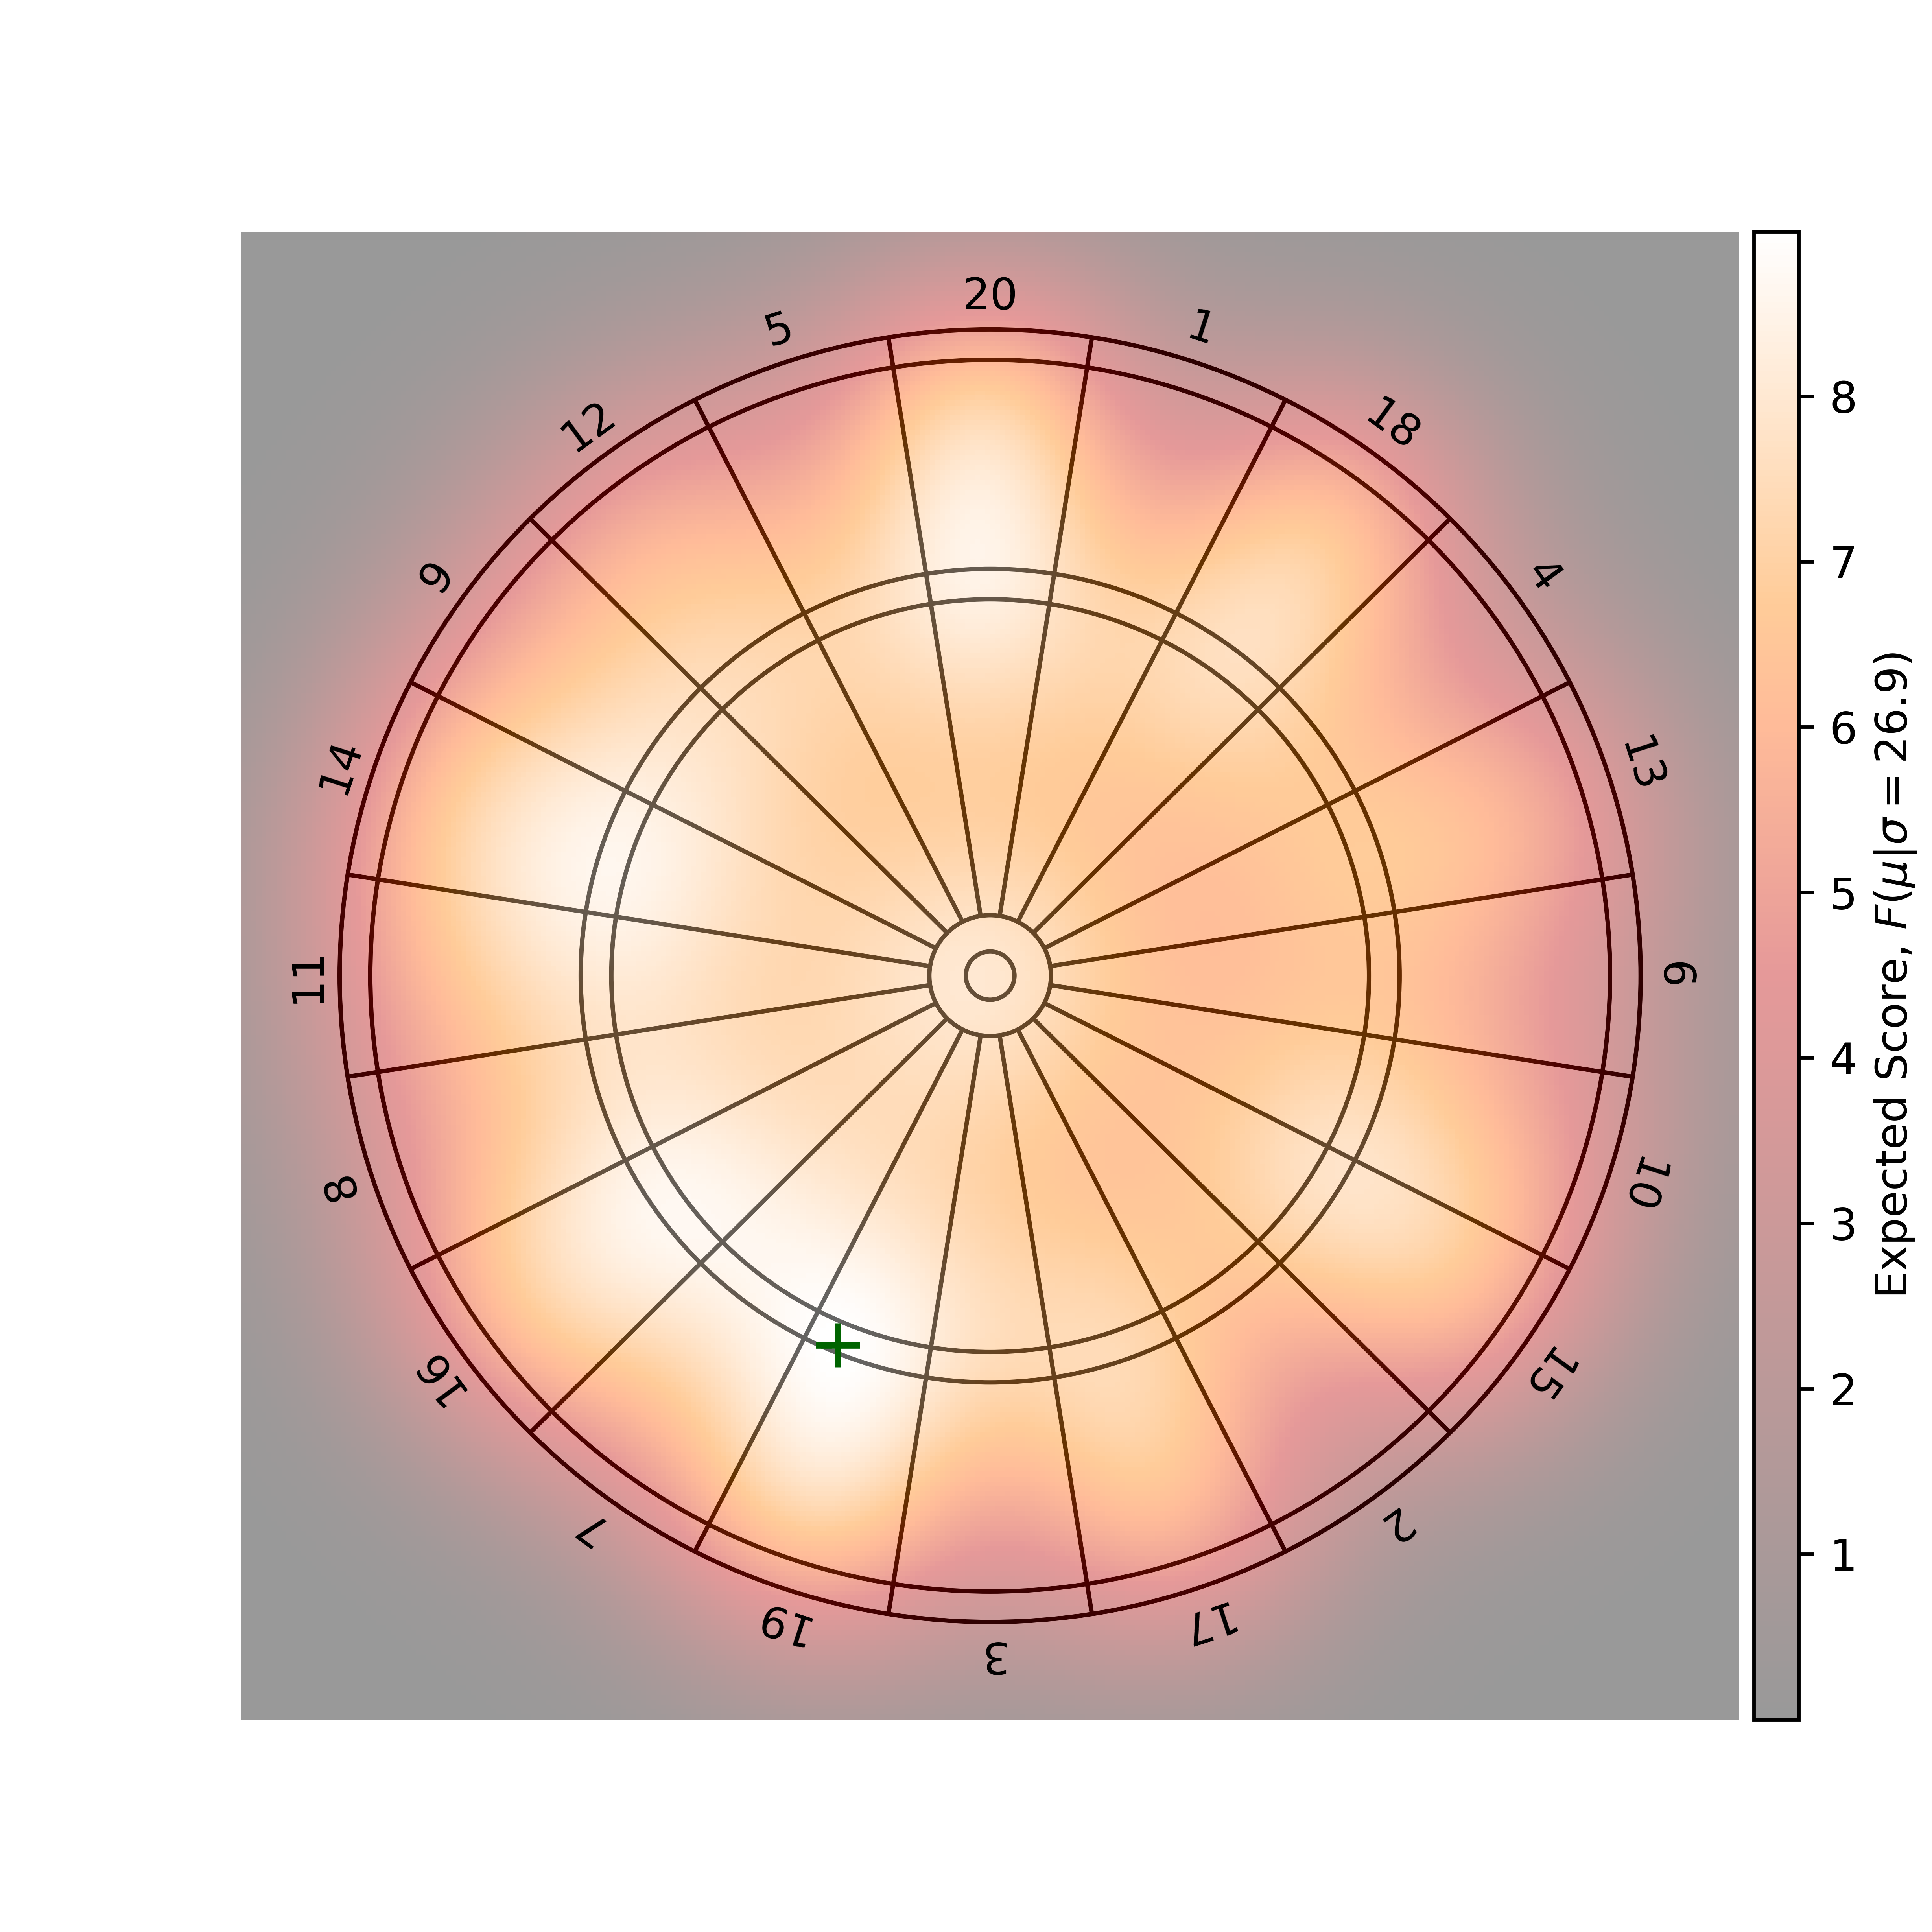
\includegraphics[width=0.8\textwidth]{../images/gist_hear.png}
	\caption{Heatmap for $\sigma = 26.9$. The green \textbf{+} is the location of  \mustar}
	\label{fig:basicheatmap}
\end{figure}

For each pixel in the heat map (i.e. each evaluation of \fmusig), I needed to compute 82 double integrals, and this method is painfully slow (see Section \ref{sec:timing} for exact numbers).


\section{Basin-Hopping}

I looked for faster ways to compute  \mustar for a fixed $\sigma$. We can think about the computation as a global maximization problem for a function of function of two inputs (the x and y coordinates of $\mu$), that is
\begin{equation}
	\mu^*(\sigma) = \max [F(\mu \vert \sigma)]
\end{equation}
By convention, global optimization algorithms find the \textit{minimum} of a function, so in practice we compute 
\begin{equation}
	\min[-F(\mu \vert \sigma)].
\end{equation}

SciPy has bindings for several different global minimization algorithms. I ended up settling on a stochastic algorithm called \textit{basin-hopping}. 

Each iteration of basin-hopping starts with a point (the ``currently accepted point''). The algorithm then takes a jump of a random size in a random direction. After landing at  a new point, the algorithm  moves ``downhill'' to a local minimum and compares the new local minimum with the currently accepted point. If the new minimum is lower than the previous one, it is always accepted. If it is not lower, there is a random process to decide whether or not to accept it, with lower minima being more likely to be accepted. The process then repeats, with another random perturbation, a local minimization, and a comparison with the most recently accepted point. Over time, random jumps get smaller, and the algorithm ends when a point has remained unchallenged for some number of cycles. The distribution of jump sizes, the local minimization algorithm, and the acceptance criteria for new points can all be controlled by parameters \cite{basin}. 

Figure \ref{fig:basin} shows a visualization for one run of the basin hopping algorithm
We should note that basin-hopping is not guaranteed to find the global minimum. If the random jumps never find the right ``basin'', the algorithm will return the wrong answer.
 \ref{fig:basicheatmap}.
\begin{figure}[h!]
	\centering
	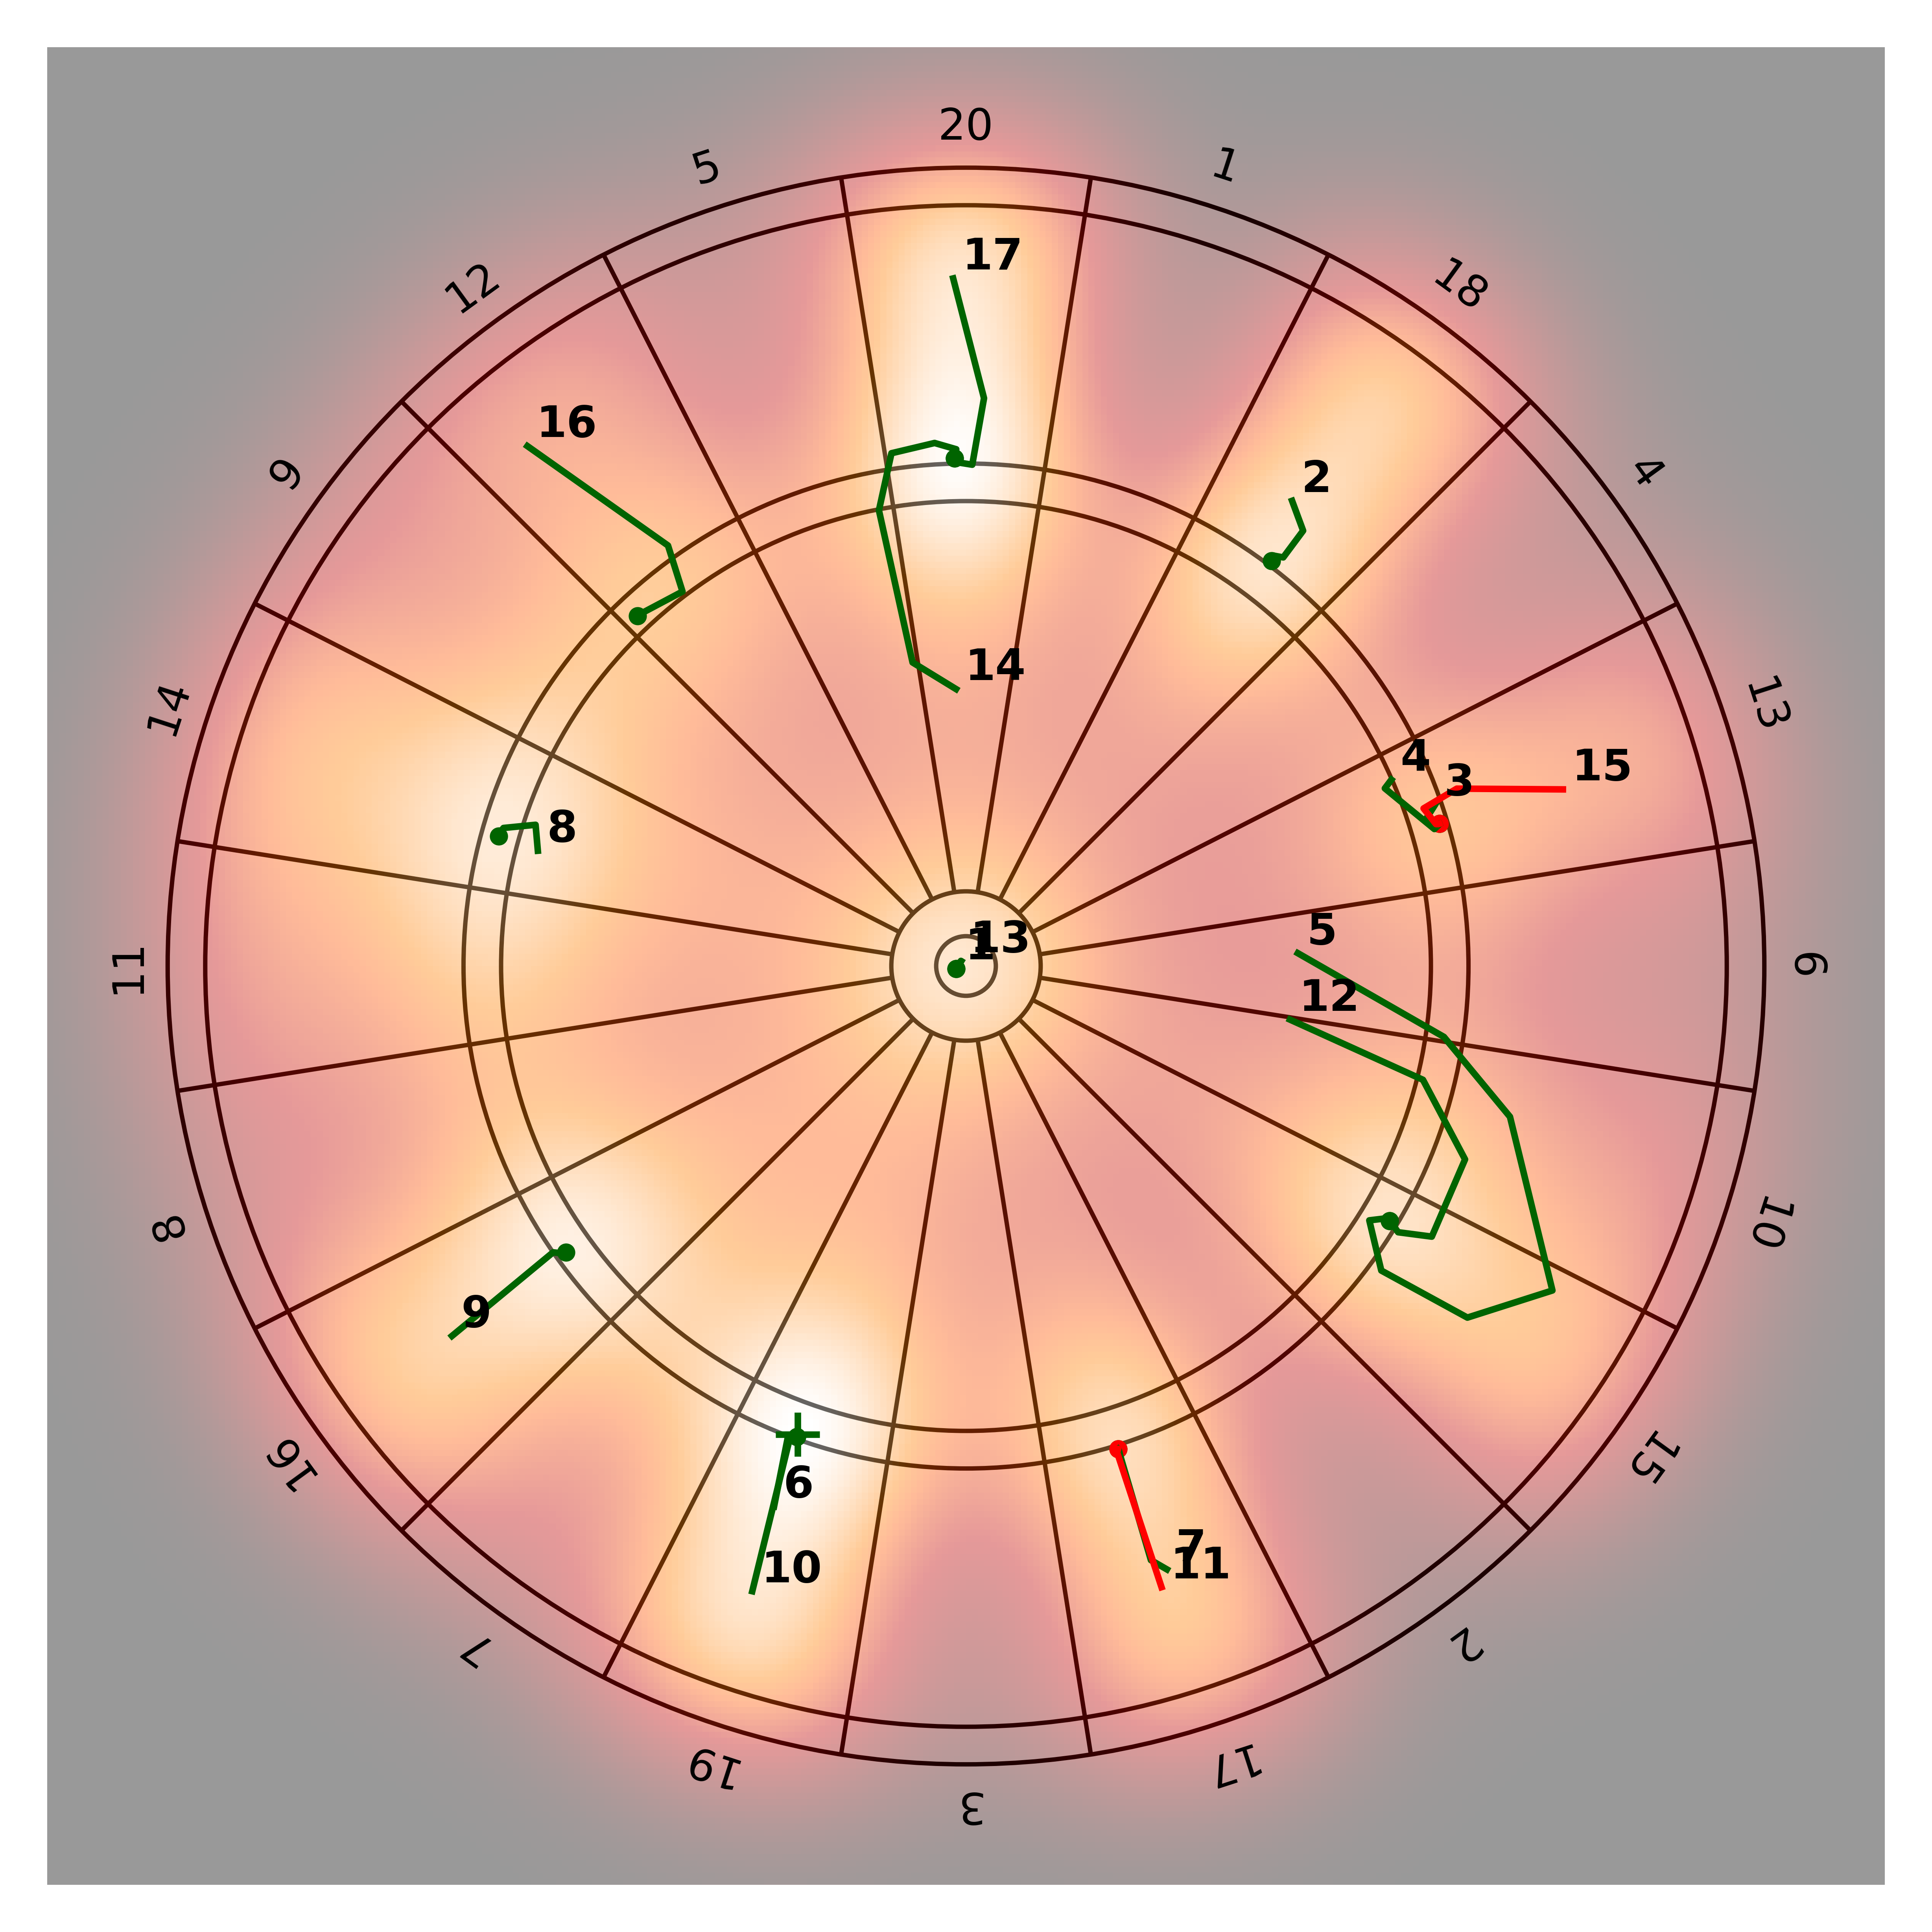
\includegraphics[width=0.8\textwidth]{../images/sig19basin.png}
	\caption{Each run of the local optimizer for a basin-hopping run to find $\mustar(\sigma=19mm)$.  Points that were \textit{accepted} by the algorithm are green while those that were \textit{rejected} are red. The green + is the true location of \mustar.}
	\label{fig:basin}
\end{figure}

While the dartboard problem proved a good way to illustrate basin-hopping, basin-hopping was not a good way to solve my dartboard problem. Besides not being guaranteed to find the correct solution, basin hopping still relies on the slow process of integration.To be sure, it is still faster than brute force: the basin-hopping run in Figure \ref{fig:basin} needed only 134 evaluations of $F(\mu \vert \sigma)$, compared to 9000 for a $300 \times 300$ heatmap. 

\section{Don't Let Ten Minutes of Reading Save You From Ten Hours of Coding}
I reread ``A Statistician Playes Darts''\cite{stat} and realized the authors came up with a much faster way to compute $F(\mu \vert \sigma)$ that I missed the first time I read the paper. The authors derived that
\begin{align}
	F(\mu \vert \sigma)  =(f_{0, \sigma^2} * score)(\mu)
\end{align}
 where $*$ is the convolution between the PDF of $\mathcal{N}(0, \sigma^2)$ and the score value for each point on the dartboard\cite{stat}. I confess I can't quite wrap my head around how this works and for the scope of this paper I will accept it as magic. Even more magical is that one can compute the convolution extremely quickly with an algorithm that uses a Fast Fourier Transform. Generating the data for a 300 by 300 heatmap such as that in Figure \ref{fig:basicheatmap} took over an hour by integration, but SciPy's \textit{fftconvolve} function gets the job done in seconds. 

\citeauthor{stat} also note that previous researchers have approximated the same results using a monte-carlo method\cite{stat}. To round off my  survey of methods for computing \mustar, I implemented the monte-carlo method. It ended up being considerably faster than direct integration even when taking many samples for each function evaluation. 

\section{Method Comparison, Timing, and Final Discussion}\label{sec:timing}

We can sum up the methods for computing in a table:

\begin{table}[h]
	\centering
	\begin{tabular}{r | c l}
		& \textbf{Deterministic} & \textbf{Stochastic} \\ \hline
		\textbf{Compute Whole Grid}& Convolution, Integration & Monte Carlo \\
		\textbf{Compute Single Point}& - & Basin-Hopping
	\end{tabular}
\end{table}

We can directly compare the speeds of those methods that compute a grid of points, paramaterizing by $n$, the side length of the grid. 

None of my homegrown methods for computing \mustar performed better than the convolution algorithm derived by \citeauthor{stat}. I think, however, that it is a valuable example of how a change in overall method can have a much greater impact than optimization within a method. 










	

\printbibliography
\end{document}
